\section{Acceptance Systematics}
\label{sec:systematic}
Systematic uncertainties arise from uncertainties on event selections expected in simulation compared to the actual performance of 
the detector. As this search is in many ways similar to the inclusive same-sign dilepton search~\cite{ssnote2011}, 
our treatment of efficiency systematics parallels the one in that analysis.
In this section, we briefly summarize those results, and
describe the uncertanities due to the b-tagging requirement.

For the inclusive search without a well-defined signal, 
we evaluate the systematics with reference to the SUSY benchmark point LM9, 
as well as opposite sign \ttbar simulation, both of which have b-enriched event topologies. The CMS benchmark point LM9 defines the 
common scalar mass (m0) $ = 1.45$ TeV, the common gaugino mass (m1/2) = 175 GeV, the ratio of the Higgs expectation
values (tan$\beta)  = 10$, tri-linear coupling (A0) = 0 and the  sign of the Higgsino mass parameter ($\mu) > 0$. This produces heavy squarks
with light gluinos leading to several heavy flavor final states.

\begin{figure}[htb]
\begin{center}
%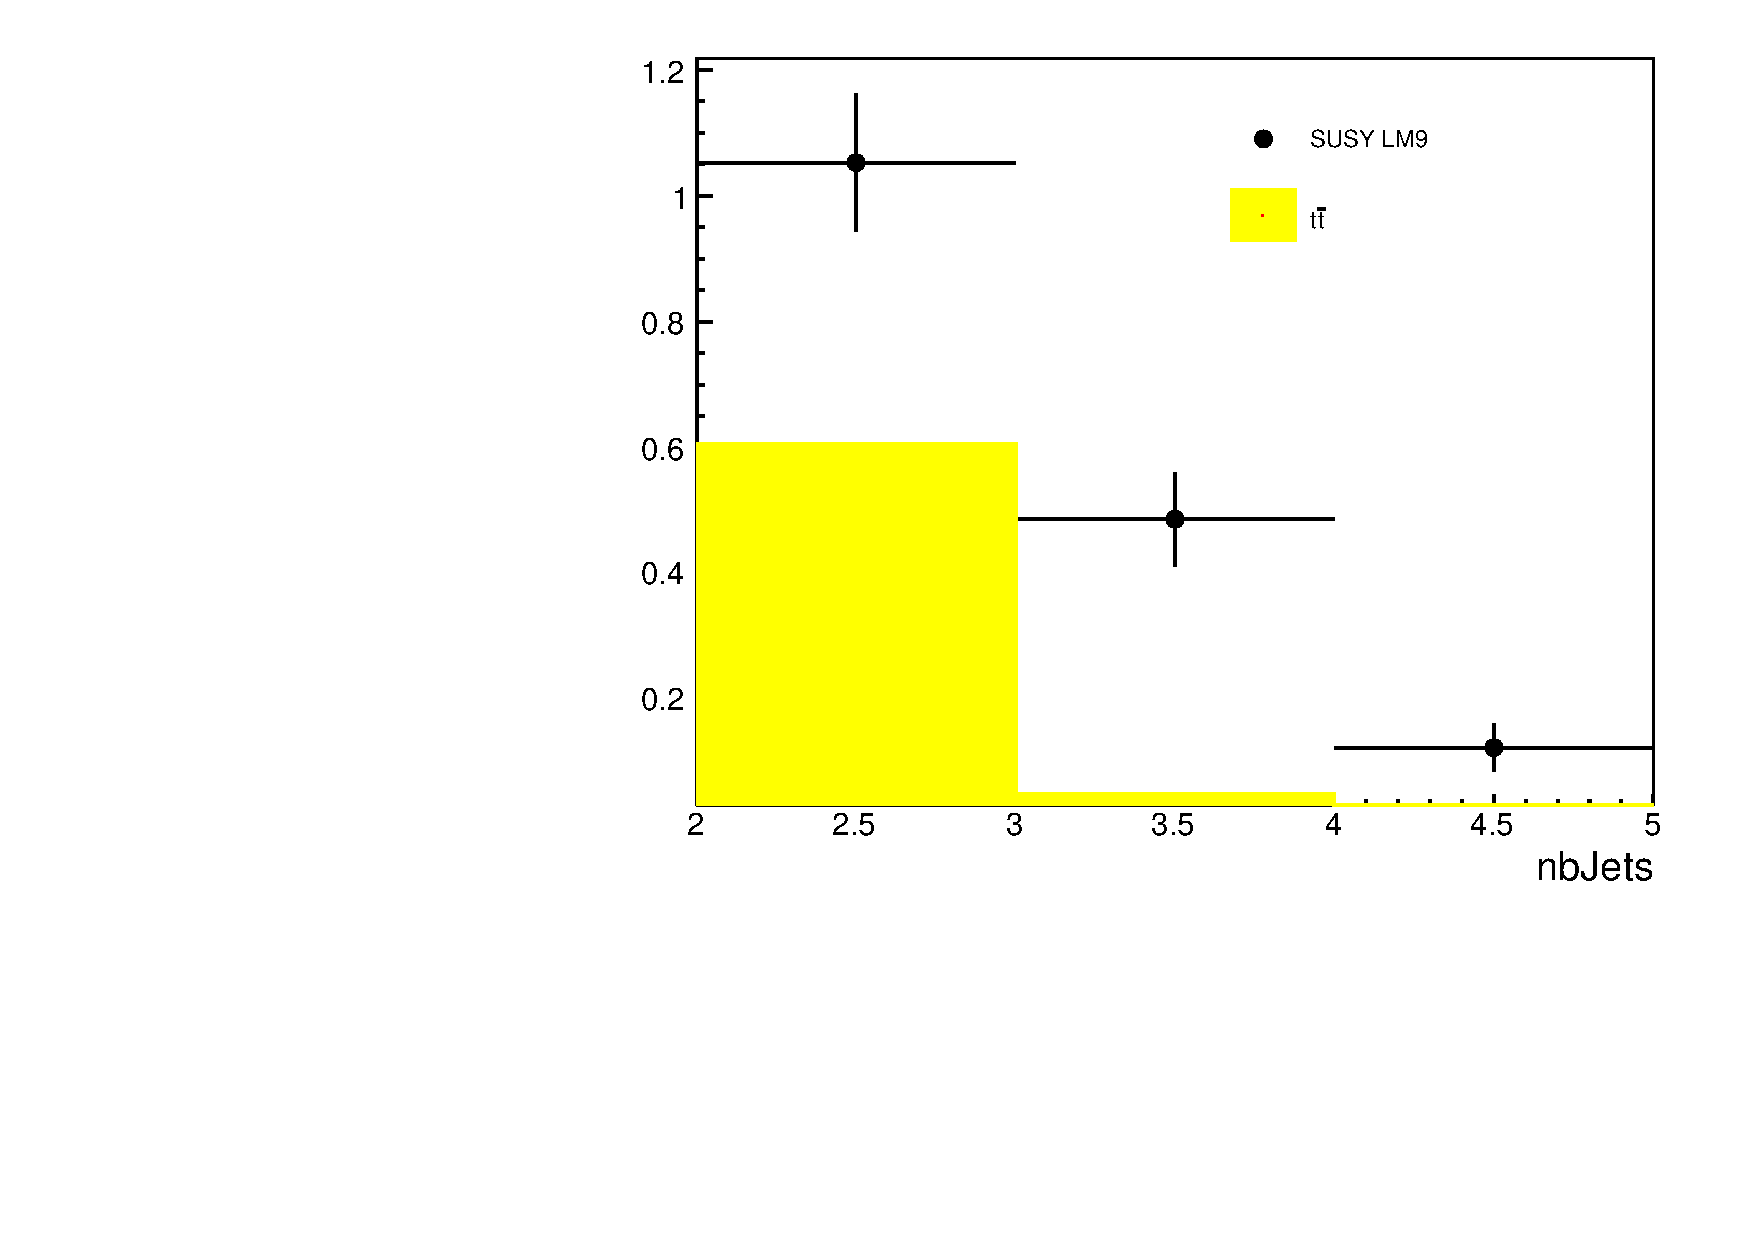
\includegraphics[width=0.48\linewidth, height=0.36\linewidth]{figs/lm9.pdf}
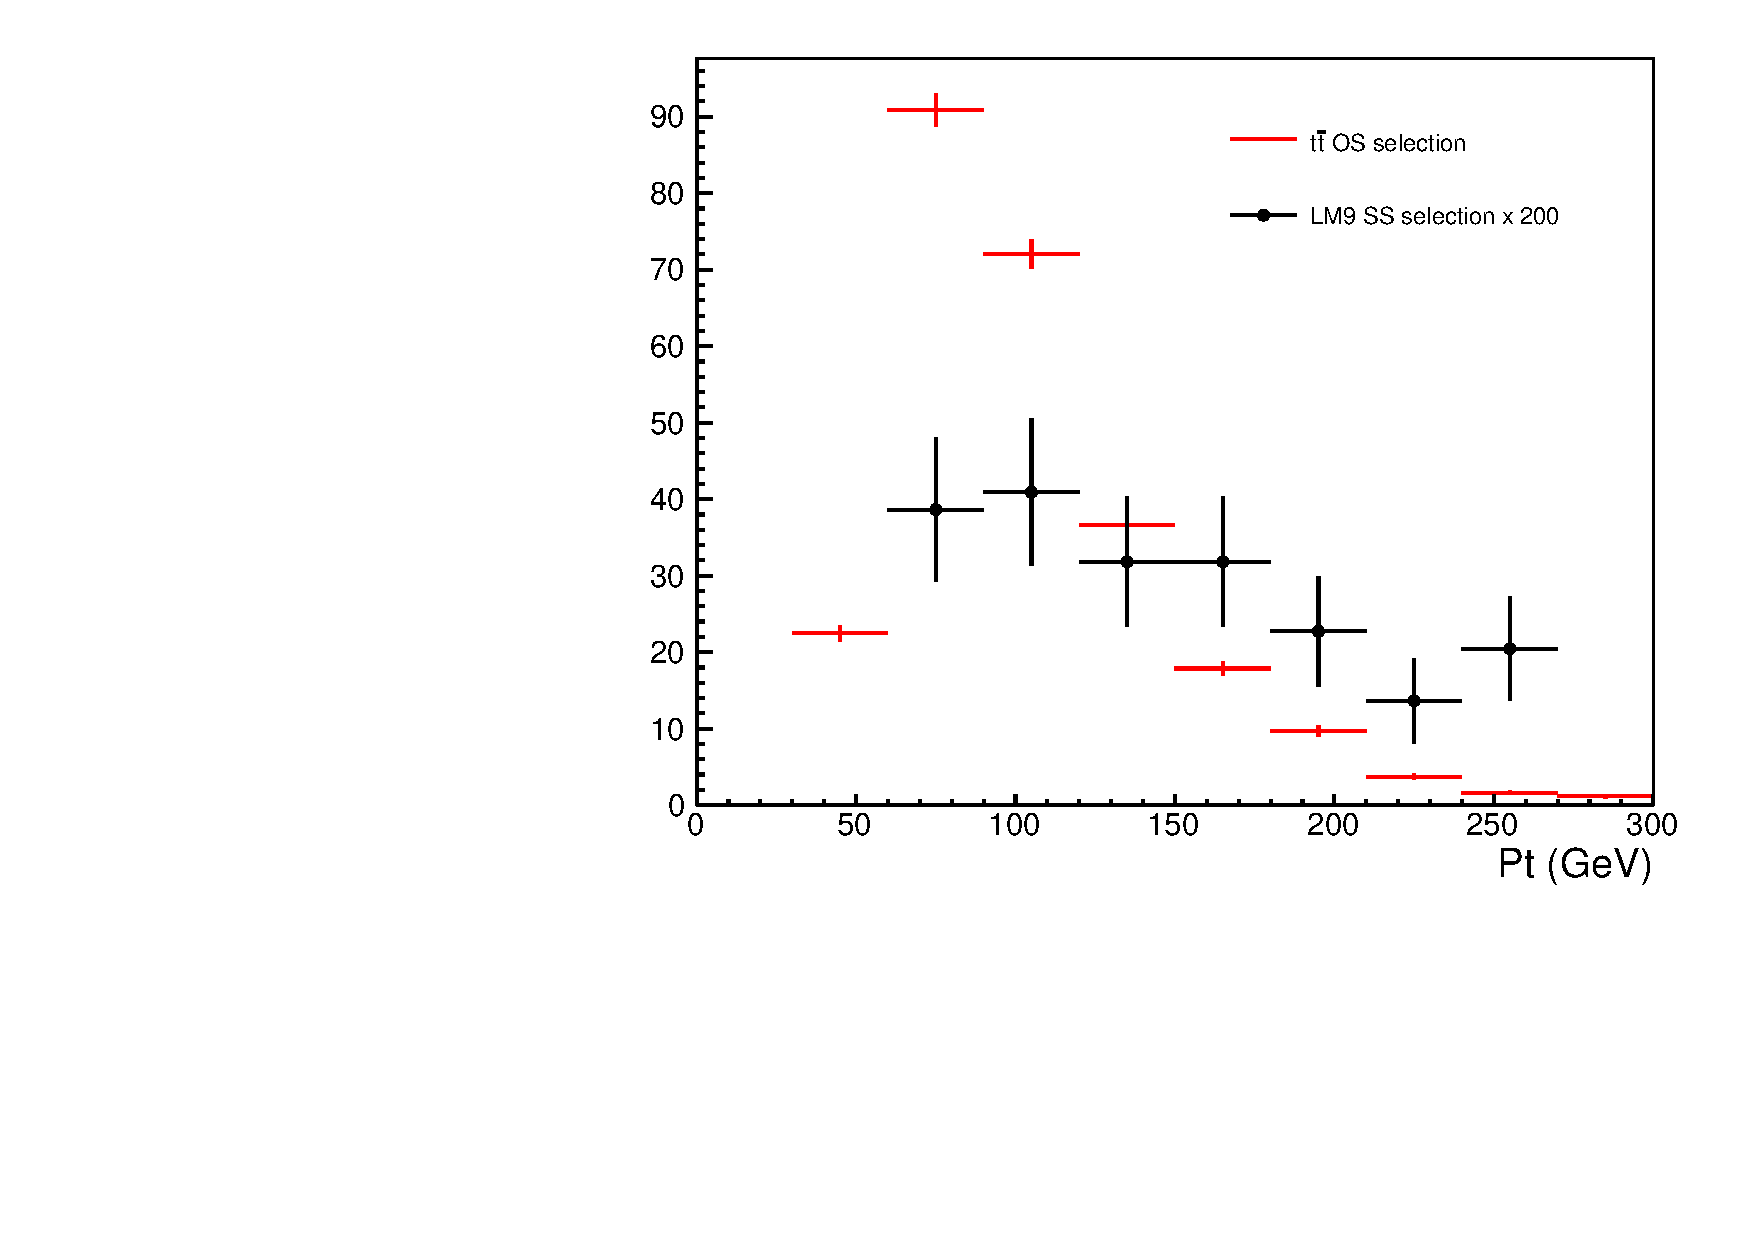
\includegraphics[width=0.6\linewidth, height=0.36\linewidth]{figs/bjetleading.pdf}
\caption{ Differential distributions of leading b-tag jet $p_T$ for the LM9 benchmark point and \ttbar simulations using 349 pb$^{-1}$ of luminosity normalization.\label{fig:lm9ttbar}}
\end{center}
\end{figure}

For the b-tagging efficiency as well as the systematic uncertanities we refer to the
work by the BTV POG group for 2011
data~\cite{BTVPAS2011}. In that study they provide the uncertanities on b-tagging efficiency, 
as well as scale factors ($SF$) for \ttbar events. In Fig.~\ref{fig:lm9ttbar} 
we compare the leading jet $p_T$ normalized distribution for LM9 using the same-sign dilepton selection. For the \ttbar events, we 
explicitely use opposite-sign dileptons in order to gain statistics. Given that the bulk of the $p_T$ range accessable by LM9 is also covered by the \ttbar decays, 
we consider 8.0\% as the systematic uncertanity on the efficiency (per b-jet) from PtRel measurements~\cite{BTVPAS2011}. We thus use the measurement of scale factors ($SFs$) 
for \ttbar for the inclusive search.

{\it Once we have all the various signal MCs we mention in Section~\ref{sec:stampCollecting}, we will replace
Figure~\ref{fig:lm9ttbar} with one that compares all of these models, and revisit the statement about
b-tagging systematics. It is likely that we will adopt different systematics for different models, given the
differences in jet $p_T$ for the different models.}

A complete summary of systematic uncertainties is given in Table~\ref{tab:systSumm}.

\begin{table}[h]
\begin{center}
\caption{\small\label{tab:systSumm}Summary of systematic uncertainties on the signal selection and
expectation. Reported values are fractional, relative to the total cross section. The values in parentheses are for electrons 
with $p_T$ below 20 GeV and muons with $p_T$ below 15 GeV for muons.}
\begin{tabular}{lcccc}\hline
Source 					& $ee$		& $\mu\mu$		& $e\mu$	& all \\ \hline
Lepton selection			& 11(15)\%	& 11(15)\%		& 11(15)\%	& 11(15)\% \\
Energy scale				& 5\%		& 5\%			& 5\%		& 5\% \\
ISR/FSR and PDF				& 2\%		& 2\%			& 2\%		& 2\% 	\\
b-tag selection                         & 16\%          & 16\%                  & 16\%          & 16\% \\
Total without luminosity		& 20(23)\%	& 20(23)\%		& 20(23)	& 20(23)\%\\ \hline
Integrated luminosity			& 6\%		& 6\%			& 6\%		& 6\%	\\ \hline
Total 					& 21(24)\% 	& 21(24)\% 		& 21(24)\% 	& 21(24)\% \\
\hline
\end{tabular}
\end{center}
\end{table}
